\documentclass[11pt]{article}

%% MinionPro fonts 
%\usepackage[lf]{MinionPro}
%\usepackage{MnSymbol}
\usepackage{microtype}

%% Margins
\usepackage{geometry}
\geometry{verbose,letterpaper,tmargin=1in,bmargin=1in,lmargin=1in,rmargin=1in}

%% Other packages
\usepackage{amsmath}
\usepackage{amsthm}
\usepackage[shortlabels]{enumitem}
\usepackage{titlesec}
\usepackage{soul}
\usepackage{tikz}
\usepackage{mathtools}
\usepackage{pgfplots}
\usepackage{tikz-3dplot}
\usepackage{algorithmic}
\usepackage[export]{adjustbox}
\usepackage{tcolorbox}

%% Paragraph style settings
\setlength{\parskip}{\medskipamount}
\setlength{\parindent}{0pt}

%% Change itemize bullets
\renewcommand{\labelitemi}{$\bullet$}
\renewcommand{\labelitemii}{$\circ$}
\renewcommand{\labelitemiii}{$\diamond$}
\renewcommand{\labelitemiv}{$\cdot$}

%% Colors
\definecolor{rred}{RGB}{204,0,0}
\definecolor{ggreen}{RGB}{0,145,0}
\definecolor{yyellow}{RGB}{255,185,0}
\definecolor{bblue}{rgb}{0.2,0.2,0.7}
\definecolor{ggray}{RGB}{190,190,190}
\definecolor{ppurple}{RGB}{160,32,240}
\definecolor{oorange}{RGB}{255,165,0}

%% Shrink section fonts
\titleformat*{\section}{\normalsize\bf}
\titleformat*{\subsection}{\normalsize\bf}
\titleformat*{\subsubsection}{\normalsize\it}

% %% Compress the spacing around section titles
\titlespacing*{\section}{0pt}{1.5ex}{0.75ex}
\titlespacing*{\subsection}{0pt}{1ex}{0.5ex}
\titlespacing*{\subsubsection}{0pt}{1ex}{0.5ex}

%% amsthm settings
\theoremstyle{definition}
\newtheorem{problem}{Problem}
\newtheorem{example}{Example}
\newtheorem*{theorem}{Theorem}
\newtheorem*{bigthm}{Big Theorem}
\newtheorem*{biggerthm}{Bigger Theorem}
\newtheorem*{bigcor1}{Big Corollary 1}
\newtheorem*{bigcor2}{Big Corollary 2}

%% tikz settings
\usetikzlibrary{calc}
\usetikzlibrary{patterns}
\usetikzlibrary{decorations}
\usepgfplotslibrary{polar}

%% algorithmic setup
\algsetup{linenodelimiter=}
\renewcommand{\algorithmiccomment}[1]{\quad// #1}
\renewcommand{\algorithmicrequire}{\emph{Input:}}
\renewcommand{\algorithmicensure}{\emph{Output:}}

%% Answer box macros
%% \answerbox{alignment}{width}{height}
\newcommand{\answerbox}[3]{%
  \fbox{%
    \begin{minipage}[#1]{#2}
      \hfill\vspace{#3}
    \end{minipage}
  }
}

%% \answerboxfull{alignment}{height}
\newcommand{\answerboxfull}[2]{%
  \answerbox{#1}{6.38in}{#2} 
}

%% \answerboxone{alignment}{height} -- for first-level bullet
\newcommand{\answerboxone}[2]{%
  \answerbox{#1}{6.0in}{#2} 
}

%% \answerboxtwo{alignment}{height} -- for second-level bullet
\newcommand{\answerboxtwo}[2]{%
  \answerbox{#1}{5.8in}{#2}
}

%% special boxes
\newcommand{\wordbox}{\answerbox{c}{1.2in}{.7cm}}
\newcommand{\catbox}{\answerbox{c}{.5in}{.7cm}}
\newcommand{\letterbox}{\answerbox{c}{.7cm}{.7cm}}

%% Miscellaneous macros
\newcommand{\tstack}[1]{\begin{multlined}[t] #1 \end{multlined}}
\newcommand{\cstack}[1]{\begin{multlined}[c] #1 \end{multlined}}
\newcommand{\ccite}[1]{\only<presentation>{{\scriptsize\color{gray} #1}}\only<article>{{\small [#1]}}}
\newcommand{\grad}{\nabla}
\newcommand{\ra}{\ensuremath{\rightarrow}~}
\newcommand{\maximize}{\text{maximize}}
\newcommand{\minimize}{\text{minimize}}
\newcommand{\subjectto}{\text{subject to}}
\newcommand{\trans}{\mathsf{T}}
\newcommand{\bb}{\mathbf{b}}
\newcommand{\bx}{\mathbf{x}}
\newcommand{\bc}{\mathbf{c}}
\newcommand{\bd}{\mathbf{d}}

%% LP format
%    \begin{align*}
%      \maximize \quad & \mathbf{c}^{\trans} \mathbf{x}\\
%      \subjectto \quad & A \mathbf{x} = \mathbf{b}\\
%                       & \mathbf{x} \ge \mathbf{0}
%    \end{align*}


%% Redefine maketitle
\makeatletter
\renewcommand{\maketitle}{
  \noindent SA405 -- AMP \hfill Rader \#2.41 \\

  \begin{center}\Large{\textbf{\@title}}\end{center}
}
\makeatother

%% ----- Begin document ----- %%
\begin{document}
  
\title{Lesson 4: Max Flow}


\maketitle

The Navy is trying to transport a large number of sailors from San Diego to Norfolk using airplanes. Unfortunately, they can not do direct flights, so they must make several stops along the way. The following diagram shows the flights available and the capacity (in hundreds) of each flight. Formulate a linear program that would allow the Navy to send as many sailors as possible from San Diego to Norfolk.



\begin{center}
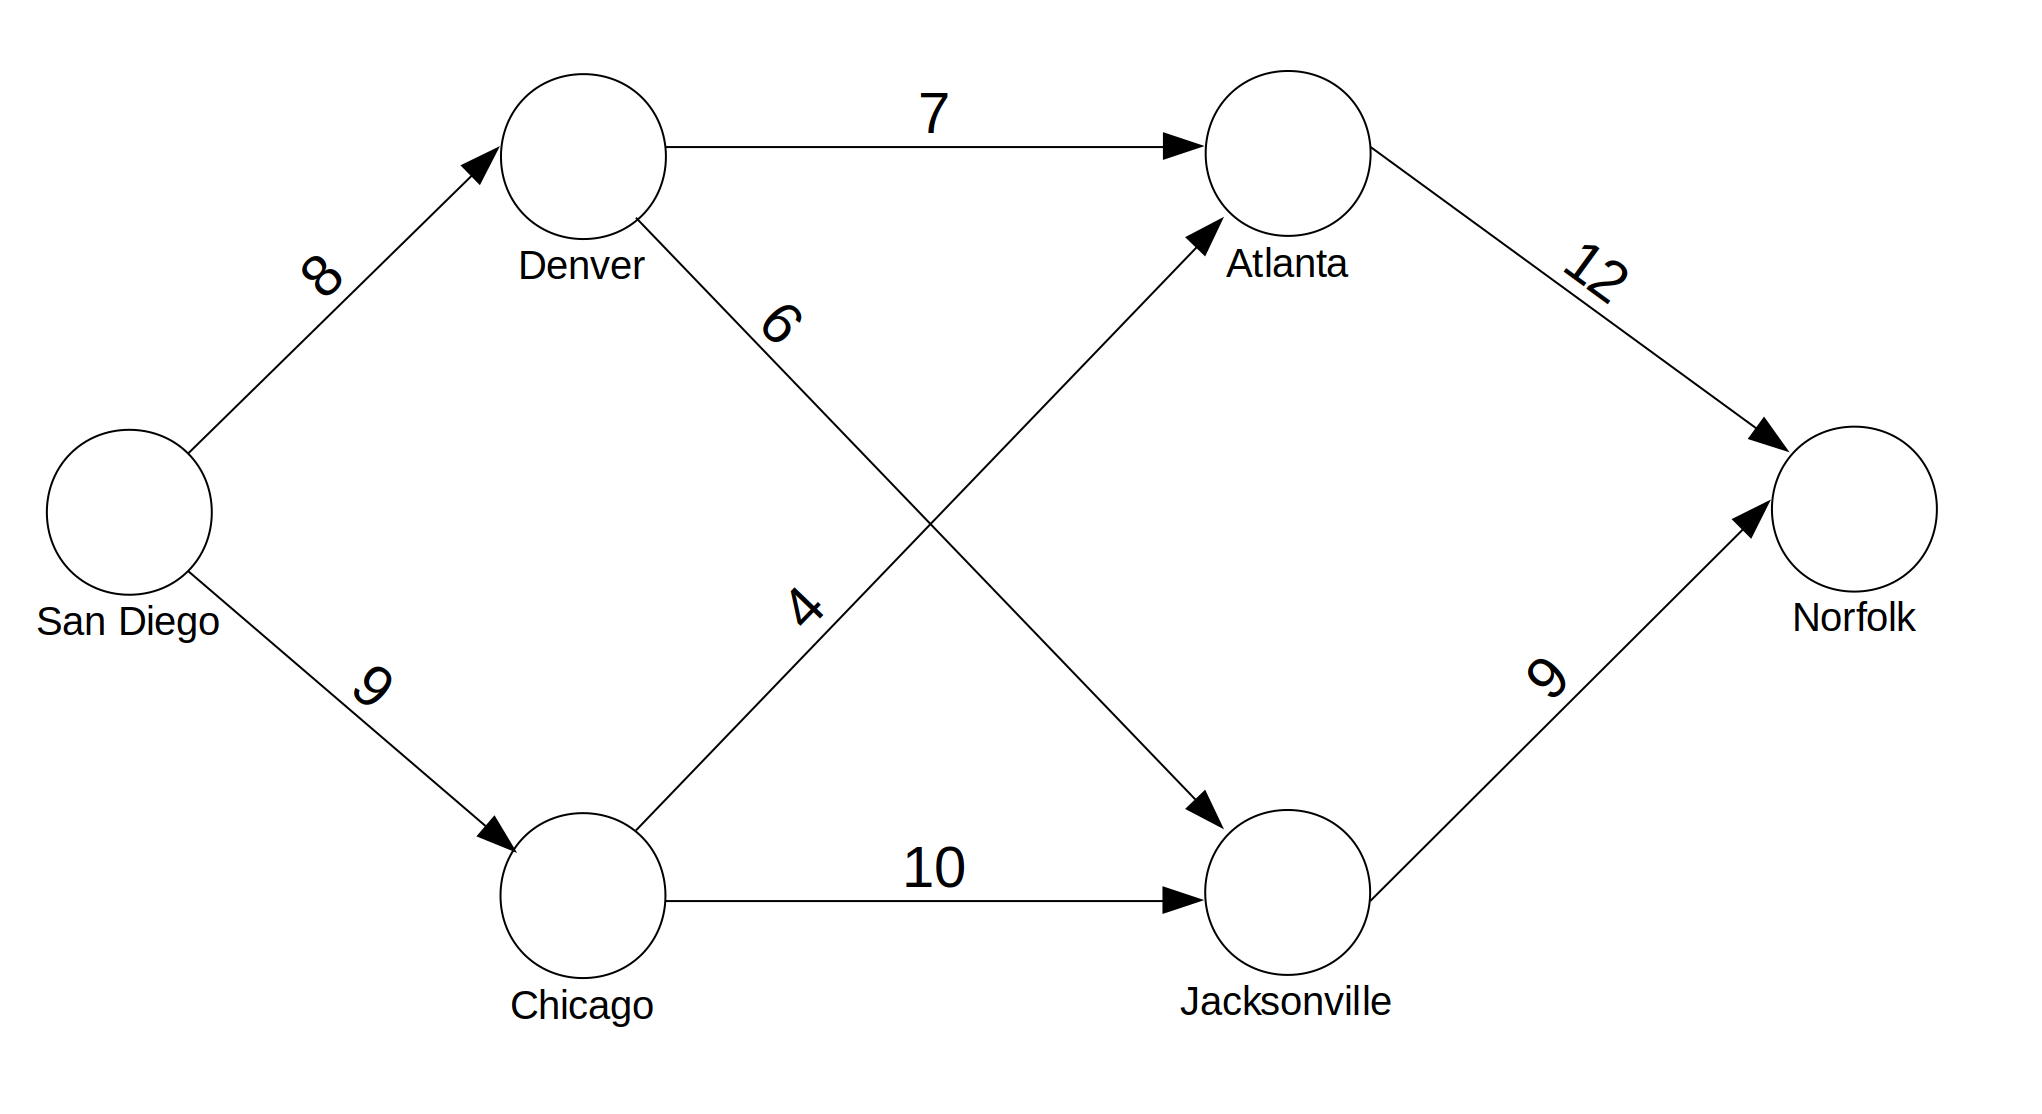
\includegraphics[width=.8\textwidth]{Military_max_flow.png}
\end{center}

Notice that these problems have a special structure. Specifically, max flow problems generally have two special nodes called the \textbf{source} and \textbf{sink} nodes.
\begin{itemize}
\item \textbf{Source node:} \vspace{1in}
\item \textbf{Sink node:} \vspace{1in}
\end{itemize}

\newpage


\begin{enumerate}
	\item It is possible to get bounds on the optimal objective function value of this problem without formulating or solving it. Based on the network flow diagram, what are some upper bounds on the max flow of this network, $z$? \vfill
	\item Based on these bounds, can you think of an equivalent minimization problem? (This is the dual problem)
	\vfill
	\item This problem does not specify supply or demand. How can we write balance of flow constraints for this problem? (Hint: there are two correct ways to do this).
	\vfill
\end{enumerate}

Before we formulate this problem, there's a couple of Theorems that are important to conclude our study of basic network problems.

\begin{itemize}
\item Max Flow Integrality Theorem \vfill
\item Min Cost Integrality Theorem \vfill
\end{itemize}

\begin{tcolorbox}
The remainder of the network problems that we study do not have this nice property so they must be formulated as an IP.
\end{tcolorbox}

\newpage


\begin{enumerate}[resume]
\item Formulate the concrete LP associated with this max flow model. \newpage
\item Generalize your LP model to a parameterized model. 
\end{enumerate}



\end{document}
